\chapter{Inferring Duplications and Losses}\label{chap:dli}

The evolution of Eukaryotic genes is largely shaped by three principal factors:
speciation, duplication and loss. First of all, speciation differentiates genes into descendants.
The story of each gene family also reflects the history of species. When an ancestor species speciates,
all of its genes will be separated into two clades at the same time and evolve
almost independently. Whereas speciations do not create new genes, duplications add
more genes to a species and the descendant species as well, and thus provide
candidates for natural selection. When more redundant genes come into being, 
losses, which tend to occur following a duplication, eliminate copies that are
of little importance to the species. Genes evolve, birth and die, telling the
complete history of individual gene families\footnote{LGT (Lateral Gene Transfer)\index{LGT, Lateral Gene Transfer},
which is thought to occur between viruses, and to a lesser extent between
prokaryotes, is also a possible factor in interpreting a gene tree. However, LGT seldom
occurs among Eukaryotes~\cite{stanhope01,salzberg01,roelofs01,frickey04}.}.
Figure~\ref{fig:exa-dup-loss} shows an example of how duplications and losses shape
the evolution of genes. If we take the duplication/loss inference presented by the tree,
the history of this gene family follows. In the earliest ancestral species {\it Chordata} there was only
one gene. It underwent a duplication in the ancestral species {\it Euteleostomi}, and since then
it had two copies in each species descendant from {\it Euteleostomi}.
The first copy evolved normally except for two succesive duplications in {\it mouse},
the second was lost in {\it Eutheria} subclass. This is the story reflected by this gene tree.

\begin{figure}[!hb]
\begin{center}
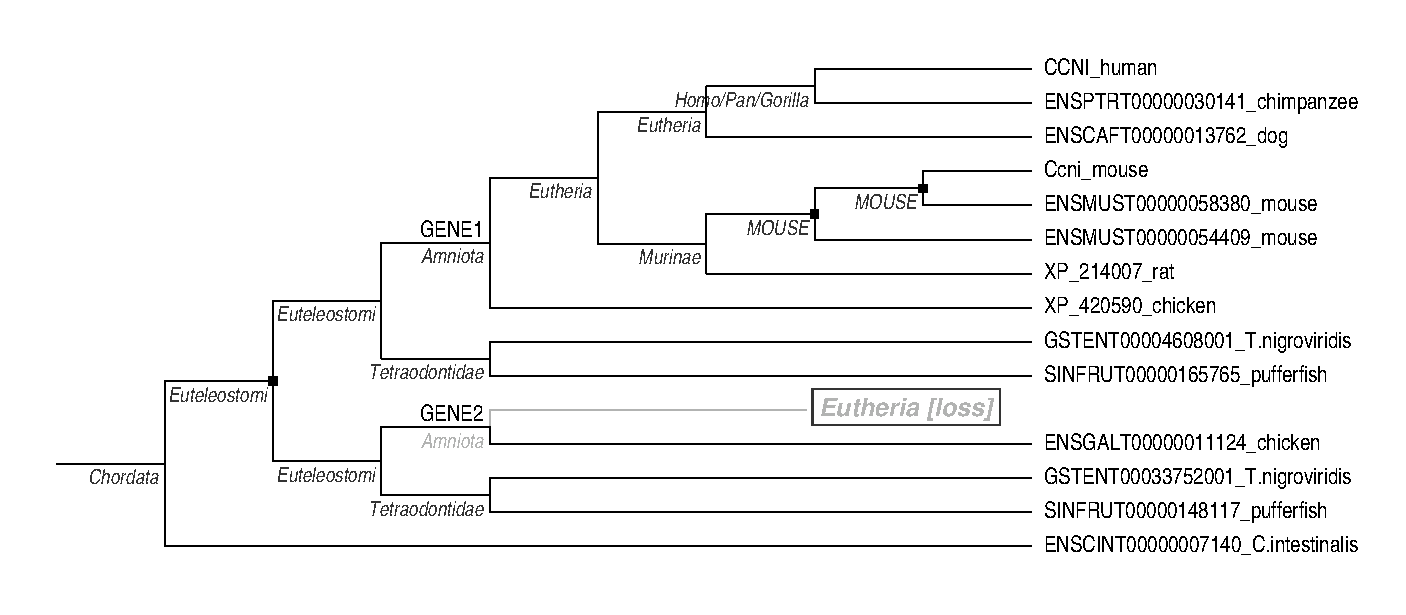
\includegraphics[width=\textwidth]{gtree}
\caption[Example of gene evolution]
{Example of gene evolution. A slant name beside an internal node
shows the ancestral species that contained the correponding ancestral gene. They are
actually $M^*(g)$ for each $g$ under parsimonious species map (Section~\ref{sec:specmap}). Duplications (the three bold nodes) and
loss (the gray boxed name) are inferred using methods that will be described in this chapter.}\label{fig:exa-dup-loss}
\end{center}
\end{figure}

The only way to infer duplications and losses is to compare the gene tree
to the species tree (Figure~\ref{fig:spectree}). This process is usually called \emph{tree reconciliation}\index{tree!tree reconciliation}
which was first suggested by Goodman~\cite{goodman79}, and implemented and improved by
many successors~\cite{page94,guigo96,eulenstein98}.
Recently, Zmasek and Eddy~\cite{zmasek01} have presented an elegant algorithm that greatly
simplifies duplication inference. Dufayard {\it et al.}~\cite{dufayard05} further developed
algorithms that could handle multifurcated species trees, though no detail is
provided. All these algorithms can be classified as parsimonious methods in
that the number of duplications and losses is minimized. A Bayesian method~\cite{arvestad03}
was also developed, which is claimed to be more effective in reducing missing duplication events.

In this chapter, we will introduce a generalized theory for duplication/loss inference,
and develop simple algorithms for such inference in the meantime. Our methods are based
on Zmasek and Eddy's work, but generalized in case of loss inference and
multifurcated species trees.

\section{Species Map}\label{sec:specmap}

To describe the inference of duplication/loss, it is necessary to bridge a gene tree
and a species tree. This bridge is called \emph{species map}\index{species map} that maps a gene, whether present or ancestral,
to the species that historically possessed the gene. When we know to which species a gene belonged,
we could pinpoint species evolution and gene evolution, reconstruct the history,
and smoothly infer the duplications and losses.

Mathematically, let $G$ be a gene tree, and $S$ a species trees, both \emph{rooted}.
Given $g\in V_E(G)$, a present gene, let $s_g\in V_E(S)$ be the species of gene $g$.
A map $M:V(G)\rightarrow V(S)$ is called a \emph{species map} if it satisfies the following
conditions for any $g\in V(G)$: (i) $M(g)=s_g$ if $g\in V_E(G)$, (ii) $s_{g'}\leq M(g)$ for all
$g'\in\omega_G(g)$ and (iii) $M(g)\leq M(g')$ if $g<g'$. Map $M$ embeds a species tree into
a gene tree and describes how the evolution of species shapes gene evolution.
In the following section, we will see that $M$ alone determines duplications and losses, and
thus how to choose $M$ is the key to duplication/loss inference.

\begin{figure}[!hb]
\begin{center}
\includegraphics{mpfig.4}\\*
\includegraphics{mpfig.5}
\end{center}
\caption[Example for illustrating species map]{Example for illustrating species map.
The top figure shows the parsimonious species map $M^*$ between species tree $S$ and gene tree $G$. Under
this map, each gene evolved normally. No duplication or loss occurred.
The bottom shows another species map $M'$ for the two trees. Under $M'$, at
least one historical duplication (at node $g'$) and two losses (showed in dashed branches)
occurred in this gene family. Note that in this example, branch length has no meanings.}\label{fig:specmap-exa}
\end{figure}

Given a specified gene tree and species tree, many maps will satisfy the two conditions.
Likelihood methods choose the one that maximizes the likelihood under certain statistical
model. This process is extremely time-consuming. In contrast, parsimony methods simply select the
the parsimonious species map\index{species map!parsimonious species map} $M^*$ that will lead to fewer duplications or losses in the end.
Without any proof here, we point out that $M^*$ can be simply constructed as:
\begin{equation}\label{equ:par-M}
M^*(g)=\lhlca(\{s_{g'}:g'\in\omega_G(g)\})
\end{equation}
Obviously $M^*$ is a species map, and in fact, $M^*(g)$ is the most recent
possible species to which $g$ belonged in history. Partly, this is also a reason why
$M^*$ is called a parsimonious map. Figure~\ref{fig:specmap-exa} gives an example of a parsimonious map and a common one.

\section{Duplication/Loss Inference (DLI)}

Ideally, a duplication can be observed if one species appears two or more times in
a gene tree. This is true if no loss occur. But when loss occur, this will overlook duplications.
We must recover the lost genes before we make such inference. For a binary species tree,
we can simply compare $M(g)$ and $M(\lhparent(g))$~\cite{zmasek01}, and infer $\lhparent(g)$ as a duplication
if $M(g)=M(\lhparent(g))$; for a multifurcated tree, however, this rule will
overestimate duplication events. As showed in Figure~\ref{fig:sigma}, both $g$ and
$g_p\equiv\lhparent(g)$ are mapped to {\it Eutheria}, but $g_p$ still represents speciation event, not
duplication. In order to generalize DLI (duplication/loss inference)\index{DLI, duplication/loss inference}
in case of a multifurcated species tree, it is helpful
to explicitly recover the species that are lost in gene trees.

\begin{figure}[!hb]
\begin{center}
\includegraphics{mpfig.3}
\end{center}
\caption[Example to explain $\sigma(g)$ set]{Example to explain $\sigma(g)$ set. In the left is a species tree $S$
with a multifurcated node; in the right is a gene tree $G$ with a loss. Node $g\in V(G)$
is mapped to $M^*(g)$ under the parsimonious map $M^*$, and $g_p$ mapped to $M^*(g_p)=M^*(g)$.
In this example,
$\sigma'(g)=\{{\it Human,Rat}\}$, $\sigma(g)=\{{\it Human,Mouse,Rat}\}$ and
$\omega_S(M^*(g))=\{{\it Human,Mouse,Rat,Dog}\}$. They are all different from one another:
$\sigma'(g)$ is smaller than $\sigma(g)$ because the mouse gene is lost,
while $\omega_S(M^*(g))$ is bigger because $M^*(g)$ is a trifurcation.}\label{fig:sigma}
\end{figure}

Given this fact, we introduce new notations:
\begin{equation}\label{equ:sigma0}
\sigma'(g)=\{s_{g'}:g'\in\omega_G(g)\}
\end{equation}
and
\begin{equation}\label{equ:sigma}
\sigma(g)=\sigma'(g)\cup\left\{s\in V_E(S):\mbox{$\exists s'\in\sigma'(g)$, $\lhlca(s,s')<M(g)$}\right\}
\end{equation}
While $\sigma'(g)$ only consists of present species that can be observed in the tree,
the second set in Equation~\ref{equ:sigma} also includes lost species in $G|_g$ subtree.
As a consequence, set $\sigma(g)$ consists of the species that should appear in $G|_g$ if no loss occurs in
this subtree.

Although the definition of $\sigma(g)$ looks complicated, it is irreplaceable.
This can be seen from the relation between the three sets $\sigma'(g)$, $\sigma(g)$ and $\omega_S(M(g))$:
$\sigma'(g)\subset\sigma(g)\subset\omega_S(M(g))$ where $\sigma'(g)=\sigma(g)$
stands if no loss occurs, while $\sigma(g)=\omega_S(M(g))$ if $M(g)$ is a binary node.
Figure~\ref{fig:sigma} also gives a concrete example where the three sets are different. As we will see in the following text,
$\sigma(g)$ plays a critical role on DLI.

\begin{figure}[!hb]
\begin{center}
\includegraphics[width=0.7\textwidth]{dli-exa}
\caption[Example of duplication/loss inference]
	{Example of duplication/loss inference. A slant name beside each internal node
	indicates the ancestral speices that contained the corresponding ancestral gene.
	Gray colour and slant leaves show the genes that cannot be observed nowadays due to loss events.
	In this gene tree, $\sigma(\mbox{\sf G1\_rat})=\{\mbox{\it Rat}\}$, $\sigma(\mbox{\sf G2\_chicken})=\{\mbox{\it Chicken}\}$,
	$\sigma(g_0)=\{\mbox{\it Huamn, Mouse, Rat, Chick}\}$ and $\sigma(g_1)=\{\mbox{\it Human, Mouse, Rat}\}$.
	Node $g_1$ is a speciation, and therefore $\lhloss(\mbox{\sf G1\_rat})=\lhloss'(\mbox{\sf G1\_rat})=\{\mbox{\it Mouse}\}$, while
	$g_0$ is a duplication and
	$\lhloss'(\mbox{\sf G2\_chicken})=\sigma(g_0)\setminus\sigma(\mbox{\sf G2\_chicken})=\{\mbox{\it Human, Mouse, Rat}\}$
	which makes $\lhloss(\mbox{\sf G2\_chicken})=\{\mbox{\it Eutheria}\}$.}\label{fig:dli-exa}
\end{center}
\end{figure}

\subsection{Inferring duplications and orthologs}

If $g\in V_E(G)$ is a duplication and no loss occurs in $G|_{g_1}$ and $G|_{g_2}$,
$\lhchild(g)=\{g_1,g_2\}$, we would expect to see $\sigma'(g_1)=\sigma'(g_2)$.
If losses occur, however, it is possible that $\sigma'(g_1)\cap\sigma'(g_2)=\emptyset$.
In this case, $\sigma(g)$ will play its role due to its inclusion of the lost species.
Formally, $g$ is a {\emph duplication}\index{duplication} (or duplication occurred at $g$) if
$\sigma(g_1)\cap\sigma(g_2)\neq\emptyset$, where $\lhchild(g)=\{g_1,g_2\}$. Figure~\ref{fig:dli-exa}
shows an example.

Orthologs are genes in different species that originate from a single gene in the last
common ancestor of these species~\cite{remm01}. Accordingly, in a gene tree, two present genes $g_1$ and
$g_2$ are said to be {\emph orthologs}\index{ortholog} if $\lhlca(g_1,g_2)$ is not a duplication.
This simple condition exactly capture the meaning of biological definition.

\subsection{Inferring losses}

We next seek to find a set $\lhloss(g)\subset V(S)$ that consists of species in which
gene losses occur when $g_p\equiv\lhparent(g)$ evolved into $g$. Note that
in this way, $\lhloss(g)$ will actually be localized at the branch between $g_p$ and $g$.
Thus the calculation at one node will not interfere with the calculation at another one, and
the total number of loss events in the tree $G$ is simply the sum of $|\lhloss(g)|$ of each node $g\in V(G)$.

As duplication and speciation represent different biological events, whether
$g_p$ is a duplication or not makes a little difference.
If $g_p$ is a duplication, subtree $G|_{g_p}$ and $G|_g$ should in theory consist of
same species. When this is violated, losses must happen and
$s\in\sigma(g_p)\setminus\sigma(g)$ covers all the species in which gene
losses occur. If $g_p$ is a speciation, besides the condition $s\in\sigma(g_p)\setminus\sigma(g)$,
a lost $s$ must appear only in $M(g_p)$'s subtree containing $M(g)$, or equivalently,
must satisfy $\lhlca(s,M(g))<M(g_p)$. We denote by $\lhloss'(g)$ the set of
present species that are lost in the gene tree\footnote{Given two sets $A$ and $B$,
$A\setminus B=\{a:\mbox{$a\in A$, and $a\notin B$}\}$.}:
\begin{equation}\label{equ:loss1}
\lhloss'(g)=\left\{\begin{array}{ll}
	\sigma(\lhparent(g))\setminus\sigma(g) & \mbox{if $\lhparent(g)$ is a duplication} \\
	\left\{s\in\sigma(\lhparent(g))\setminus\sigma(g):\lhlca(s,M(g))<M(\lhparent(g))\right\} & \mbox{otherwise}
	\end{array}\right.
\end{equation}
Set $\lhloss'(g)$ consists of present species that cannot be observed due to losses between $g$ and $g_p=\lhparent(g)$.
However, this is not good enough. A loss of ancestral species will cause the losses of
all the descendant present species. Based on parsimonious rule, we would like to count this as one loss event.
For this purpose, we define:
\begin{equation}\label{equ:loss2}
\lhloss(g)=\{s\in V(S):\omega_S(s)\subset\lhloss'(g),\omega_S(\lhparent(s))\not\subset\lhloss'(g)\}
\end{equation}
Set $\lhloss(g)$ avoids over-counting. It is actually the minimum set $A\subset V(S)$ satisfying $\omega_S(A)=\lhloss'(g)$.
Also take Figure~\ref{fig:exa-dup-loss} as an example. In this gene tree,
$\lhloss'(${\sf ENSGALT00000011124\_chicken}$)=\{\mathit{human,mouse,rat,dog}\}$ and
$\lhloss(${\sf ENSGALT00000011124\_chicken}$)=\{\mathit{Eutheria}\}$. {\it Eutheria} is just the species where the loss occured.
Figure~\ref{fig:dli-exa} gives another example.

\section{Duplication Function and Loss Function}\label{sec:dl-fun}
Both duplication function and loss function are defined on $V_I(G)$:
\begin{eqnarray}\label{equ:dl-fun}
D_G(g) &=& \left\{\begin{array}{ll}
	1 & \mbox{if $g$ is a duplication} \\
	0 & \mbox{otherwise}\end{array}\right. \\
L_G(g) &=& \sum_{g'\in\lhchild(g)}{|\lhloss(g')|}
\end{eqnarray}
Duplication function $D_G(g)$ measures whether $g$ is a duplication; loss function $L_G(g)$
counts losses when $g$ evolved into its children. Obviously, the total number of duplications and
losses in gene tree $G$ simply equal to $\sum D_G(g)$ and $\sum L_G(g)$ respectively.
Given a common species map $M$, the definitions of duplication and loss
functions must depend on the topology of the gene tree $G$, but if parsimonious species map
$M^*$ is applied, duplication and loss functions can be topology-independent.
This will be re-examined in Section~\ref{sec:re-dl-fun} when set representation is introduced.

\section{Towards Statistical Methods}

\begin{figure}[!hb]
\begin{center}
\includegraphics{mpfig.11}
\caption[Example showing the failure of parsimonious species map]
{Example showing the failure of parsimonious species map. Assume the
the true history of gene evolution included one duplication at {\it Eutheria} and two losses in
{\it Murinae} and {\it Human}. The human gene and the mouse gene are not orthologs. Arbitrarily applying the
parimonious species map $M^*$ will always miss these events and wrongly infer the two genes as orthologs.}\label{fig:bad-pars}
\end{center}
\end{figure}

In this section, we will come back to the selection of species map $M$ that
uniquely determines how the duplication and loss are inferred. Usually we only take
the parsimonious species map $M^*$ due to its simplicity, but unfortunately nature does not always
follow the parsimonious rule. In a multigene family
where duplications and losses tend to occur frequently, arbitrarily choosing $M^*$ might
underestimate the numbers and lead to more orthologs (Figure~\ref{fig:bad-pars}). More
sophisticated method that could possiblely select the species map other than $M^*$
should be applied this time. A Bayesian method has been introduced by
Arvestad {\it et al.}~\cite{arvestad03,arvestad04} and cleverly solve this problem.
We do not intend to present detailed description, which is far beyond the
scope of this thesis. We only add more remarks in comparison of parsimonious $M^*$ and
$M$ favoured by Bayesian method.

In Bayesian framework, the desired species map is the one that maximize the posterior
probability $\Pr\{M|G,S\}$, which can be calculated as:
\begin{eqnarray*}
\Pr\{M|G,S\}&=&\frac{\Pr\{M,G|S\}}{\Pr\{G|S\}}\\
	&=& \frac{1}{\Pr\{G|S\}}\cdot\int_{\mu}\int_{\lambda}\Pr\{M,G,\mu,\lambda|S\}\,d\mu\,d\lambda \\
	&=& \frac{1}{\Pr\{G|S\}}\cdot\int\!\!\!\int\Pr\{M,G|S,\mu,\lambda\}\Pr\{\mu,\lambda|S\}\,d\mu\,d\lambda \\
	&=& \frac{1}{\Pr\{G|S\}}\cdot\int\!\!\!\int\Pr\{M,G|S,\mu,\lambda\}p(\mu,\lambda|S)\,d\mu\,d\lambda \\
\end{eqnarray*}
where $\lambda$ is the birth rate, $\mu$ is the loss rate and
$p(\mu,\lambda|S)$ is the prior probability of $(\mu,\lambda)$ given a species tree $S$.
When no prior knowledge is available, we usually take bounded uniform distribution as what Arvestad {\it et al.}
has done. In this equation, $\Pr\{G|S\}$ is a constant given a specified $G$. Then all we should do
is to calculate $\Pr\{M,G|S,\mu,\lambda\}$. If we assume that when separated, whether by speciation or duplication,
genes evolved independently, $\Pr\{M,G|S,\mu,\lambda\}$ can be written as
the product of a series of independent factors\footnote{$M^{-\!1}:V(S)\rightarrow 2^{V(G)}$ can be regarded ass the reverse
of species map $M$.}:
\begin{equation}
\Pr\{M,G|S,\mu,\lambda\}=\prod_{s\in V(S)}\,\prod_{g\in M^{-\!1}(\lhparent(s))}q_G(g,s)
\end{equation}
where $q_G(g,s)$ is the probability of forming the observed gene tree when a single gene $g$ of $\lhparent(s)$ evolved into
its descendants of species $s$. Thus $\prod_{g\in M^{-\!1}(\lhparent(s))}q_G(g,s)$
represents the probability of forming the observed gene tree when species $\lhparent(s)$ evolved into $s$.
As to the calculation of $q_G(g,s)$, Arvestad {\it et al.} presents detailed descriptions base on previous works~\cite{nee94,yang97}.

%To demonstrate the advantage of Bayesian methods, Arvestad {\it et al.} showed two examples:
%the first was an MHC multigene family which contained many duplications
%and losses; the second example contained fewer duplications and losses, but they claimed that
%Bayesian method could give better support values. While the first example was appropriate, the second
%might be misleading. This can be accounted for by two reasons. First, the authors used
%MrBayes~\cite{huelsenbeck01} to generate, or reconstruct,  possible gene trees, and Bayesian method tends to yield `excessively high' support
%values~\cite{suzuki02,cummings03,simmons04}. And second, in their benchmark,
%both RIO~\cite{zmasek02} and OrthoStrapper~\cite{storm02} reconstruct resampled trees by Neighbour-joining that might be
%less accurate in comparison to likelihood method~\cite{kuhner94}. This will lead to lower support values, too.
%If RIO and OrthoStrapper had also inferred orthologs from gene trees reconstructed by MrBayes,
%they would probably have got similar support values.

Bayesian method establishes an elegant framework for tree reconciliation and also for
various complex analyses about gene evolution, including reconstructing species trees and gene trees
with the help of each other~\cite{arvestad04}.
However, Bayesian method might be faced with a few theoretical difficulties both in biological angle and
in mathematical angle. First of all, separated genes, either by duplication or speciation events, did not
evolve independently. Losses tended to occur after massive duplications. One-copy genes were also less likely to
be lost. These facts are not modeled in Bayesian framework at present.
Furthermore, Bayesian method has to work with
a prior distribution, which can improve the accuracy when correctly formed but may also induce bias when not carefully selected.
Unfortunately, bounded uniform distribution of $\lambda$ and $\mu$
is not appropriate. On one hand, from the known gene trees in TreeFam~\cite{li06},
birth rate $\lambda$ and death rate $\mu$ are centered around small values;
on the other hand, in order to deal with families with massive duplications
and losses where parsimony fails, bound values must be large enough. This produces the confliction.
Whereas the use of parsimonious map
never produces false duplications when the gene tree is correct, the use of Bayesian one will, and the use of such a uniform
distribution will further aggregate the problem because the higher probabilities
at larger $\lambda$ and $\mu$ tend to favour more duplications.
False duplications, which might cause more problems than
missing some, have to be evaluated before we apply Bayesian method in practice.

In most cases where $\mu$ and $\lambda$ are small, parsimonious species map $M^*$ is accurate enough.
Although in a complex gene family where duplications and losses frequently occurred it can be wrong, use of Bayesian method does not
give us more confidence when even the gene tree is questionable. Furthermore, under parsimonious
map duplication and loss functions also become topological independent.
These properties make $M^*$ particularly useful in Chapter~\ref{chap:merge}.
